% This is samplepaper.tex, a sample chapter demonstrating the
% LLNCS macro package for Springer Computer Science proceedings;
% Version 2.20 of 2017/10/04
%
\documentclass[runningheads]{llncs}
\newcommand{\quotes}[1]{``#1''}
\newcommand{\singlequotes}[1]{`#1'}
\renewcommand{\arraystretch}{1.5}
%
\usepackage{graphicx}
\usepackage[super]{nth}
\usepackage{mdframed}
\usepackage[most]{tcolorbox}
\usepackage{boldline} 
\usepackage[ruled,vlined]{algorithm2e}
\usepackage{mathtools}
\usepackage{algorithmic}
\usepackage{multicol}
\usepackage{verbatim}
\usepackage[colorinlistoftodos]{todonotes}
\usepackage[ruled]{algorithm2e}


\usepackage{hyperref}
\usepackage{comment}
\usepackage{amsmath,amssymb,amsfonts,amsthm}
\usepackage{mathcomp}

\renewcommand{\algorithmicrequire}{\textbf{Input:}}
\renewcommand{\algorithmicensure}{\textbf{Output:}}



\newtcolorbox[blend into=figures]{myfigure}[2][]{float=htb,
title={#2},#1}
% Used for displaying a sample figure. If possible, figure files should
% be included in EPS format.
%
% If you use the hyperref package, please uncomment the following line
% to display URLs in blue roman font according to Springer's eBook style:
% \renewcommand\UrlFont{\color{blue}\rmfamily}

\begin{document}
%
\title{Password Generation Using Bi-Directional Generative Adversarial Network\\ \quotes{BIPASSGAN}}
%
%\titlerunning{Abbreviated paper title}
% If the paper title is too long for the running head, you can set
% an abbreviated paper title here
%
\author{First Author\inst{1}\orcidID{0000-1111-2222-3333} \and
Second Author\inst{2,3}\orcidID{1111-2222-3333-4444} \and
Third Author\inst{3}\orcidID{2222--3333-4444-5555}}
%
\authorrunning{F. Author et al.}
\titlerunning{BIPASSGAN}
% First names are abbreviated in the running head.
% If there are more than two authors, 'et al.' is used.
%
\institute{Princeton University, Princeton NJ 08544, USA \and
Springer Heidelberg, Tiergartenstr. 17, 69121 Heidelberg, Germany
\email{lncs@springer.com}\\
\url{http://www.springer.com/gp/computer-science/lncs} \and
ABC Institute, Rupert-Karls-University Heidelberg, Heidelberg, Germany\\
\email{\{abc,lncs\}@uni-heidelberg.de}}
%
\maketitle              % typeset the header of the contribution
%

\begin{abstract}
The password is the most prevalent and reliant mode of authentication by date. Recent advancements in IoT have propelled various other mechanisms, but they face severe issues of hardware and software constraints. These scenarios make users rely on this old password-based authentication technique. In the age of no-privacy, human creativity has reached a limit. Passwords used and generated are not secure enough. Deep networks and adversarial created samples are mimicking the unthinkable. The overuse of social networks has exposed our user profiles, which increases risk based on individuals and demands personalized models. We have proposed a novel deep learning approach using a bi-directional generative adversarial network  \quotes{BIPASSGAN} to generate personalized passwords that may be at risk. We have used One-class SVM for determining the strength of the same.

\keywords{Password  \and Machine Learning \and Transfer Learning \and Deep Learning \and GAN \and PASSGAN \and BIGAN \and One-Class SVM}
\end{abstract}
\section{Introduction}
Passwords have been the primary source of authentication since we entered the digital age. After a long technological evolution and evolution of various other authentication techniques, we still rely on the very same passwords. This over-dependence on passwords requires human efforts and creativity for generating new ones and keeping them secure at the same time. In this machine learning and data-centric era, we often talk that privacy is a myth. With cheap computation and readily available resources, it has become effortless to crack passwords. In this paper, we will discuss the current works for guessing passwords. It introduces requirements beyond human creativity to generate secure passwords. Above all, we have thought about personalizing this scheme. The prevailing models are generalized and may prove strong for one case and weak for the other. Transfer learning can come to rescue, and users can have their personalized models. In sections below, we will briefly explain the literature and compare it with what we proposed.


The above study motivates for designing a new novel approach for generating passwords and very same time checking its performance and strength. So, why the human chosen password is still prevalent. It is easy to implement, and no specialized hardware is required. Human thinks way different beyond machines. From where passwords come from or generated. Human thinking is getting exposed over the years through excessive use of the internet. Machine and deep learning techniques have become smart enough to match our though. It has brought issues into existence that passwords have become easy to guess. We tend to use the same password as they are hard to remember and trying to type correctly. It makes the user use the same password every time. It increases the probability of attack. 

Before the advancement of machine learning and deep learning, state of the art for guessing attacks were brute force and dictionary attack. In brute-force \cite{8400211} the attacker tries all the password combinations. With this attack, guessing a password is guaranteed but not feasible because of the time taken. The other one is the dictionary attack, as the name suggests, the dictionary may be a collection of word lists which are familiar sources for users to choose mnemonic passwords.\cite{8400211} Researchers enhanced guessing attacks using probabilistic context-free grammar(PCFG).\cite{5207658} It takes the probability of the frequency of the structure of the password and guesses a password. For example, the guess "password123" may be more probable than the guess "P@ssW0rd!23" depending on the password creation policy and user creativity. In 2016, Melicher et al. proposed that neural network models that can generate human-created passwords.\cite{197243} Recurrent neural networks can learn from sequences. Researchers use Long short-term memory to avoid gradient vanishing problem. \cite{DBLP:journals/corr/Lipton15} All these machine learning algorithms work well. 

Still, they all have the same limitations as they can only generate a subset of the password possible, and it depends on the knowledge they have extracted from the leaked password. Generative Adversarial Network(GAN) has been widely used in recent years for the generation of new and unseen samples in every corner of the research. \cite{goodfellow2014generative} With the help of this generative model (Briland Hitaj, Paolo Gasti, Giuseppe Ateniese, Fernando Perez-Cruz) proposed PASSGAN.\cite{DBLP:journals/corr/abs-1709-00440} GAN takes large no of epochs and hence a long time for generating passwords. Bi-Directional GAN is an extension of GAN and performs faster in comparison. \cite{DBLP:journals/corr/DonahueKD16}. 

In GAN, we find the distribution of the data set P(w). With the help of a generator and discriminator, we try to create a distribution with noise(o), which will be similar to P(w). We faced the problem as it takes a longer time to converge the distribution. So, we used Bi Direction GAN in which by adding one more element, we can converge much faster and get satisfactory results on generating new passwords. Further, We trained a One-class SVM model for checking the strength based on all the passwords generated based on training over existing and generated passwords. And, We emphasis on personalized model training such that it proves efficient for individuals. The remainder of this paper is organized as follows. Section II discusses the Background and Related Works. Section III summarizes the methodology and briefs the preliminaries and explains the proposed work. Section IV lists the experiments and results. Section V discusses the conclusion and future work.

\section{Related Work}
\\

\subsection{\textbf{Brute-Force and Dictionary Attack:}}
\newline 

The oldest password guessing tools are brute force attack \cite{8400211} and dictionary attack \cite{8400211}. It can also be categorized as an offline and online attack. The attacker obtains the hash of the password of the target user and tries to get the plain text by guessing iteratively in an offline attack. Thousands, millions of iteration may be required. It is an example of a brute force attack where the attacker tries all possible passwords until it matched the original password. It takes an ample amount of time, and also requires a huge amount of storage. 
\par
In the dictionary attack, the attacker adds some input with a common password based on some rules and tries to guess the password adding new words systematically by applying pre-selected mangling rules. For a dictionary attack to be successful, it requires the original word to be in the attacker's input dictionary, and for the attacker to use the correct word-mangling rules. The main challenge to make offline password attacks is to generate an ordered list of password guesses p1,p2,p3,p4, and so which matches the original password. An online attack happens when the attacker uses some API to enter password guess against some account. 
\newline
\subsection{\textbf{Machine learning:}}
Many authors have proposed and studied password guessing, generation techniques. Earlier, They used brute-force techniques and lexical grammar for this purpose. With cheap resources available and advancements in deep learning, guesswork became easier. Recent models and works analyzed and emulated human thinking and creativity to generate many similar passwords as we can. Nowadays, more exposed profiles have resulted in frequent targeted attacks. It makes the recent works susceptible, ineffective, and motivates us to study them. 

Research on human chosen passwords is going on for many years. Many researchers try to learn the pattern of passwords and try to memic passwords generating new or similar kinds of passwords. Researchers used natural processing tools to generate a password. Previous tools include using Markov model \cite{Narayanan:2005:FDA:1102120.1102168} to improve the dictionary-based attack.
\newline
\\
\subsection{\textbf{Markov model:}}
\newline
Markov model is based on the Markov chain rule. Markov chain is a mathematical system in which it transits from one state to another state according to specific probabilistic rules. It has many applications in other forms. 

In password generation, this model uses the idea of a transition between the characters. For example, if we take the word \singlequotes{Alice}. If we use the Markov model of \nth{3} order then the word is divided into \singlequotes{Ali}, \singlequotes{lic}, etc. The idea of a transition between the characters itself becomes its limitation.
\begin{itemize}
\item As for the better result, we have to check all the possibilities of the order of the Markov model and choose which order Markov model is the best model.\item It reaches a lower converge rate of test passwords while generating the same length password.  \item It is hard to choose the operative word mangling rules to use for a dictionary attack.
\end{itemize}The improvement of this model omen model\cite{10.1007/978-3-319-15618-7_10} was created. By adding the ranking of passwords, it makes the guessing of passwords faster.
Then the researcher started to think about the structure of the leaked password. The researcher began to take an idea from the natural processing language and try the probabilistic context-free grammar model\cite{5207658} on creating a password and guessing the password.
\\

\subsection{\textbf{Probabilistic context-free grammar model:}} 
\newline
This approach generates password structures in the highest probability order. The word mangling rules are automatically created. It takes a keyword and multi-word pattern into account. \cite{7098389} Using PCFG in \cite{5207658} Authors observed that not all guesses have the same probability of cracking a password. For example, the theory "password12" may be more probable than the guess "P@ssW0rd!23" depending on the password creation policy and user creativity.
\newline
\\
\subsection{\textb{Neural Network:}}
\newline
Researchers also used the concept of neural networks to crack passwords. They created a Recurrent Neural Network\cite{197243}.
The recurrent neural network is a kind of neural network where the output from the previous node is the input of the next node. In the underlying neural network, input and output are independent of each other. Still, as we have to predict the next character, this neural network requires the knowledge of the previous character to predict a new character. The most crucial feature of RNN is the hidden state, which remembers the information of the sequence. The issue that has been faced by the Rnn are \begin{itemize}
    \item It faces an issue of vanishing gradient problem.
    \item It is hard to choose the best n-gram split.
\end{itemize}
It was the first neural network approach for cracking the password.
To overcome the first limitation of the Rnn model, Long short term memory is used. \cite{DBLP:journals/corr/Lipton15} A hierarchical semantic model is based on semantic analysis, which analyzes patterns and semantics of the dataset. It has been tested on the Chinese passwords dataset, which is a collection of leaked passwords from several websites, excluding CSDN passwords. The CSDN passwords are reserved for model testing. We segment passwords into meaningful words and meaningless strings. A neural network is trained with these segmented passwords. \cite{10.1007/978-981-13-5913-2_6} In 2016, Melicher et al. proposed that neural networks could model human-created passwords. They used neural networks for password strength measures. \cite{197243} In this model, each password is split in n-gram (best result when n=3), and the n-gram split data is forwarded to the recurrent neural network to generate a new password.
\newline

\subsection{\textbf{Deep Learning:}}
\newline
Generative models \cite{goodfellow2014generative}, a new sensation in deep learning, is used to generate new passwords. Generative Adversarial Network is one kind of generative model. The model consists of (a) generator and (b) discriminator that competes with each other. Real data(w) distribution is \[{P_W(w)}\] given with generated data(u) \[{P_U(u)}\] from the generator to the discriminator. The discriminator tells whether the data is real or fake and gives feedback to the generator. The generator tries to minimize the error and makes the distribution similar, which cannot be discriminated by the discriminator.
\[ \minG  \maxD  V (D, G)=E _{w \sim pdata(w)}[log D(w)] + E _{u \sim p u(u)} [log(1-D(G(u)))]. \]
\newline
\newpage
\section{Proposed Work}
\newline
In this section, we will discuss the generative model. A generative model is a kind of unsupervised model. This model has a powerful way to learn any data distribution, and it has tremendous success in recent years. In this paper \cite{goodfellow2014generative} they have tried to create a password. We have taken a new type of bi-directional Generative Adversarial Network to generate a new password. We have named the model as "BiPassGan." In this paper, we will show that our model is better than the previous proposed deep learning model. With the output of our model, we will create tools for cracking the password as well as predicting the strength of a user given password.

\subsection{Generative Adversarial Network:} It has been recently introduced to train a generative model to generated new data. It consists of two adversarial networks :(a) Generative model G that captures data distribution and (b) Discriminative model D that estimate the probability that sample have come from training data or generative model. Both G and D could be multi-level perceptron. 

In Generative adversarial network generator and discriminator play thief and police game where the generator model tries to fool the discriminator, and the discriminator try to discriminate. Initially, the discriminator discriminates easily, but as the round increases generator network started to update its parameter.
\newline
\\
\textbf{Generator Model:}~~ The main motive of this model is to generate the input distribution as real as possible. Eg-if, we take an image from the data set this model to try to learn so that it creates a realistic image representation of actual data.
\newline
\textbf{Discriminate Model:}~~ The main motive of this model is to identify the fake image produced by the generator from the real data.
\newline
\hfill \break
\subsection{Working Principle of GAN and k is the least expensive option}
\begin{algorithm*}[H]
%\hspace{-0.5 cm}
%\centering
\caption{Setup}
\label{algo:pre}
%\begin{multicols}{2}
%\underline{{\footnotesize \textbf{Sender's Payment Routine:}}}
%\vspace{-0.4 cm}
\begin{algorithmic}[1]
%\REQUIRE ($S \rightarrow u_1 \rightarrow \cdots \rightarrow u_i \rightarrow \cdots \rightarrow u_n \rightarrow R$, $v$)
%\ENSURE
%\vspace{0.2 cm}
    
    \FOR{$\emph{~no of training iteration} $}
         \FOR{$\emph{k steps}$}
            \STATE \emph{sample m noise sample from noise prior{$P_U(u)$}}
            \STATE \emph{sample m example from data  {$pdata(w)$}}
            \STATE \emph{update the discriminator by ascending its stochastic gradient}
        \ENDFOR
        \STATE \emph{sample m noise sample from noise prior ${P_U(u)}$}
        \STATE \emph{update the generatorby its stochastic gradient}
    \ENDFOR
    \STATE \emph{the gradient based updates can use gradient based learning rule}

 \caption{Algorithm of GAN and k is the least expensive option}    
\end{algorithmic}
%\end{multicols}
%\vspace{-0.3 cm}
\end{algorithm*}

\subsection{\textbf{GAN training process:}}
\newline
\begin{itemize}
  \item we take some noise from a random distribution and feed it to the generator. 
  \item, we take the generated image and real image to discriminator alternatively.
  \item the discriminator is a binary classification neural network, so it calculates loss for both the fake data and real data and combines them to find the total loss.
  \item The generator G also calculates the loss from its noise as Gloss.
  \item both the loss is sent to their respective network to adjust their parameter.
  \item Apply any optimization algorithm, we have used Adam Optimizer.
\end{itemize}
\newline
\subsection{\textbf{GAN`s Objective function:}}
\newline
\begin{itemize}
    $o\rightarrow Noise Vector$\ ~~~ $G(o)\rightarrow Generator~  output$\
    \newline
    $w\rightarrow Training~sample$\ 
    \newline
    $D(w)\rightarrow Discriminator~ output~ for~ real ~(0,1) $\
    \newline
    $D(G(o))\rightarrow Discriminator~ output~ for~ fake ~(0,1) $\
    \newline
    \newline
    \textbf{At Discriminator:}
    \newline
    \begin{itemize1}
        \item $D(w)\rightarrow ~maximized$\
        \newline
        \item $D(G(o))\rightarrow ~minimized$\
    \end{itemize1}
    \newline
    \newline
    \textbf{At Generator:}
    \begin{itemize}
        \newline
        $D(G(o))\rightarrow ~maximized$\
    \end{itemize}
    
\end{itemize}
\textbf{Loss Function:}
\newline
\textbf{At Discriminator D:}
\newline
\begin{itemize}
$Dloss_{real}=log(D(w))$\
\newline
$Dloss_{fake}=log(1-D(G(o)))$\
\newline
$Dloss=Dloss_{real}+Dloss_{fake}~=~log(D(w))+log(1-D(G(o)))$\
\newline
the total cost is 
\newline
\( \frac{1}{m} \) $\sum_{i=1}^{m} log(D(w^i))+log(1-D(G(o^i)))$ 
\end{itemize}
\newline
\newline
\textbf{At Generator G:}
\newline
\begin{itemize}
$Gloss=log(1-(D(o))) ~or~ -log(D(G(o)))$\
\newline
the total cost is 
\newline
\( \frac{1}{m} \) $\sum_{i=1}^{m} log(1-(D(o^i)))$
or
\newline
\newline
\( \frac{1}{m} \) $\sum_{i=1}^{m} -log(D(G(o^i)))$
\end{itemize}
\newline
\textbf{Total Loss of GAN:}
\[ \minG  \maxD  V (D, G)=E _{w \sim pdata(w)}[log D(w)] + E _{o \sim p o(o)} [log(1-D(G(o)))]. \]
\subsection{\textb{Bi-directional GAN:}}
Bi-directional GAN just extends the GAN by adding the third component. The third component is the encoder. The work of the encoder is to map the data from data space w to latent space o.The objective of the generator remains the same whereas the objective of the discriminator is altered to classify between the real sample and the fake sample and additionally between a real encoding and a fake encoding.
\newline
\textbf{Generator(Decoder):}
\newline
Assume that we have a prior belief on where the latent space o lies:\[{P_O(o)}\] Given a draw from this latent space the generator G, a deep learner, outputs a synthetic sample.
\[ G(o|\theta_G):o\rightarrow w_{synthetic}\]
\newline
\textbf{Encoder:}This is the inverse of the generator. From a given data space the encoder E outputs a real encoding.\[ E(w|\theta_E):w \rightarrow o\]
\textbf{Discriminator:}The discriminator classify if a sample is from the real data distribution.
\[{P_W(w)}\] \\ or the synthetic data distribution \[P_G(w|o)\]\\ classify whether an encoding is real \[ P_E(o|w)\] \\ or synthetic \[P_O(o) \]
\textbf{BIGAN Objective Function:}
\newline
\begin{equation*}
\min_{G(o;\theta_G),E(w;\theta_E)}  \max_{D[(w,o);\theta_D]}V(D[(w,o):\theta_D],G(o;\theta_G),E(w;\theta_E)=
\end{equation*}
\begin{equation*}
E_{w\sim P_{W}(w)}E_{o\sim P_{E}(o/w)}log[D[(w,o); \theta_D ]]+
\end{equation*}
\begin{equation*}
E_{o\sim P_{O}(o)E_{w\sim P_{G}(w/o)}}log[1-D[(\^{w},o); \theta_D ]]
\end{equation*}
\subsection{Working Principle of BiGAN}
\begin{algorithm*}[H]
%\hspace{-0.5 cm}
%\centering
\caption{Setup}
\label{algo:pre}
%\begin{multicols}{2}
%\underline{{\footnotesize \textbf{Sender's Payment Routine:}}}
%\vspace{-0.4 cm}
\begin{algorithmic}[1]
%\REQUIRE ($S \rightarrow u_1 \rightarrow \cdots \rightarrow u_i \rightarrow \cdots \rightarrow u_n \rightarrow R$, $v$)
%\ENSURE
%\vspace{0.2 cm}
    
    \FOR{$\emph{~no of training iteration} $}
         \FOR{$\emph{k steps}$}
            \STATE \emph{Some noise is chosen from random distribution}
            \STATE \emph{That noise is given to the generator to generate data
 and also offered to the decoder to create synthetic encoding.}
            \STATE \emph{Real data is given to the encoder to generate real encoding.}
            \STATE \emph{All the four-element are given to the discriminator to classify between an actual sample and a synthetic sample and additionally between an actual encoding and synthetic encoding.
 }
            \STATE \emph{update the discriminator by ascending its stochastic gradient}
        \ENDFOR
        \STATE \emph{sample m noise sample from noise prior ${P_U(u)}$}
        \STATE \emph{update the generator by its stochastic gradient}
    \ENDFOR
    
 \caption{Algorithm of BIGAN}    
\end{algorithmic}
%\end{multicols}
%\vspace{-0.3 cm}
\end{algorithm*}
\subsection{Dataset Preprocessing and Feature Extraction}
\textbf{Password data set:}
The data we have used to generate a new password is the leak RockYou data set. We have taken a 10,00,000 password. we split ed the data in 80 percent for training and the remaining 20 percent for testing.
%need a table with a most frequent password and their occurrence
\newline
\\
\textbf{Data cleaning:}
Many data in the data set are still in the hash value. Many passwords are repeated, and many are contain non-ASCII characters .we have to remove the non-ASCII character from the data set. Their many passwords of the length of 4 characters. We have taken the mini mun password size six and the maximum password of 14 characters. The most common password around a 60 percent password contains lower case letters.
\newline
\\
\textbf{Data conversion:}
{As we split the data set into two-part (a) Training (b) Testing. We take the training data and convert it into an image of the 7*maximum size of the password. To make the dimension of all images the same, we set maximum size as 14 by padding space.First we have taken all the number(0-9),upper case character(A,B,..Z),lowercase character(a,b,c,..,z) and special character(@,+,-,&..) total 92 including space.Assign every character of the password with a number. Then we have taken each character from a password and take it decimal representative and convert it into a 7-bit binary representation. We have done this work for all the passwords in the training set.

\par
\newline
\begin{table}[h]
\centering
\caption{Representing text into binary }
\label{}
\scalebox{0.7}{
\begin{tabular}{||c||c||}
    \hline
    \hline
    \textbf{Password} & \textbf{ Binary Representation} \\
    \hline \hline
    sanjay & '0110110', '0100100', '0110001', '0101101', '0100100', '0111100' \\
    \hline
    sandip & '0110110', '0100100', '0110001', '0100111', '0101100', '0110011' \\
    \hline
     rockyou  & '0110101', '0110010', '0100110', '0101110', '0111100', '0110010', '0111000' \\

    \hline
     devil & '0100111', '0101000', '0111001', '0101100', '0101111' \\
    \hline
     passwor & '0110011', '0100100', '0110110', '0110110', '0111010', '0110010', '0110101' \\
     \hline
     Riya & '0011011', '0101100', '0111100', '0100100' \\
    \hline
    123456 & '0000001', '0000010', '0000011', '0000100', '0000101', '0000110' \\
    \hline
    8820337820 &~'0001000', '0001000', '0000010', '0000000', '0000011', '0000011', '0000111', '0001000', '0000010', '0000000'\\
    \hline
    \hline
\end{tabular}}
\end{table}
}
\subsection{Training Bigan:}
We trained our Bigan model with the train password data, which we have converted into an image with a dimension of 7*maximum size of the password i.e., 14 in our case. We turned each password into an image and fed it to the discriminator with the decoder of it as well as the generated image with its vector representation alternatively.
It took 6 hrs to train the model on the RockYou data set with batch size 64 on the Ubuntu cluster. 

\subsection{Creating Password using BipassGAN}
After the password image is given to the Bigan, the model trains itself and generates a picture with a dimension of 7*14 as output. During the generation, the value range from 0 to 1.To make it as binary representation, we give a threshold in which less than 0.5 will be represented as 0 and greater as 1. Then we take 7 bit sequentially and convert the binary representation to decimal. Then with the help of our character to decimal representation, we turn the decimal to its character representation. As all the passwords will be of 14 sizes because we padded with space.so after the generation of the password, we remove the padded space from the password. In our experiment, we have taken 64 batch sizes with Adam optimizer with a learning rate of 0.002.

\section{Result:}
\newline
{{After the generation of passwords, with the help of set theory, we can find a unique password generated by the model. First, we take all the test data into a set to find the unique test password. Then we compare the generated password with the test data.we have significant results compared to the first deep learning approach.
\newline

\begin{table}[htb]
\centering
\caption{Result of passgan using the Rockyou data set in 199000 iterations}
\label{}
\scalebox{0.8}{
\begin{tabular}{||c||c||c||}
    \hline
    \hline
    \text{Password Generated} & \text{Unique Password} & \text{Password Matched(1978367 unique sample)}\\
    \hline
    \hline
    10^4 & 9738 & 103(0.005)\\
    \hline
    10^5 & 94400 & 975(0.048)\\
    \hline
    10^6 & 855972 & 7543(0.381)\\
    \hline
    10^7 & 7064483 & 40320(2.038)\\
    \hline
    \hline
\end{tabular}}

\end{table}


\par
\begin{table}[htb]
\centering
\caption{Result of bipassgan using the My space data in 160000 iteration}
\label{}
\scalebox{0.8}{

\begin{tabular}{||c||c||c||}
    \hline
    \hline
    \text{Password Generated} & \text{Unique Password} & \text{Password Matched(145588 unique sample)}\\
    \hline
    \hline
    10^4 & 9878 & 247(0.16)\\
    \hline
    10^5 & 97323 & 112(0.76)\\
    \hline
    10^6 & 971712 & 6234(4.28)\\
    \hline
    10^7 & 8732545 &32571(22.3)\\
    \hline
    \hline
\end{tabular}
}
\end{table}

\par
\newline
\begin{table}[htb]
\centering
\caption{Result of bipassgan using the rockyou data set in 160000 iteration}
\label{}
\scalebox{0.8}{

\begin{tabular}{||c||c||c||}
    \hline
    \hline
    \text{Password Generated} & \text{Unique Password} & \text{Password Matched(145588 unique sample)}\\
    \hline
    10^4 & 9978 & 287(0.18)\\
    \hline
    10^5 & 99473 & 1334(0.87)\\
    \hline
    10^6 & 978976 & 7318(4.78)\\
    \hline
    10^7 & 8324568 &39648(25.8)\\
    \hline
    \hline
\end{tabular}}
\end{table}

\newline
\begin{figure}[ht!] %!t
\centering
\begin{mdframed}
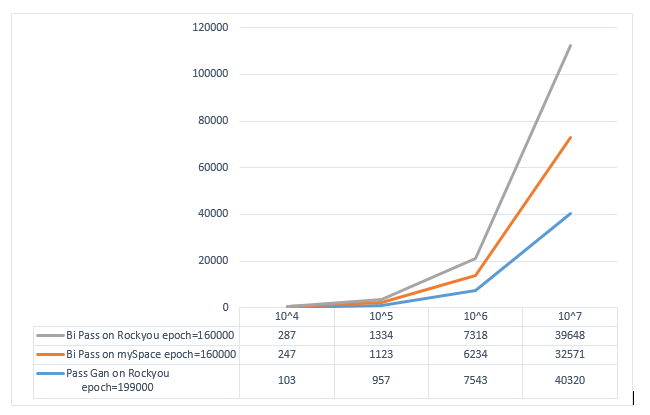
\includegraphics[width=4 in]{Compare.png}
\end{mdframed}
\caption{Compare Between PASSGAN AND BIGAN}
\label{LP}
\end{figure}
\newline
}
}
\newline
\section{Password Strength Evaluation:}
\subsection{Related Work:}
With the advancement of the neural network, the researcher used the neural network for measuring the strength of the password.\cite{197243} as we know the password the oldest and still the most frequently used authentication method. A password strength estimator can significantly help the user to choose a strong password. Tools till now are only tested on the English language and not tested on any other language. In this paper,\cite{article}, they have adapted the password strength meter in the Czech language. They have changed the zxcvbn estimation engine for the Czech and Slovak languages.
There is much research going on the policy of password creation. In this paper, \cite{GUO2019423}the researcher has found a password policy known as optiwords, which is easy to remember by the user.  Optiwords is a new textual password creation policy that is based on picture superiority effect, which provides users with a direct "drawing-to-text" method for creating user-friendly passwords. Password strength meter depends on the amount of training dataset available in this paper \cite{Guo2018LPSELP}. They have proposed a lightweight password strength meter is known as LPSE: Lightweight password-strength estimation. In this model, they make a vector representation of the password and compare their cosine similarity and edit distance between the password. Based on the cosine similarity and edit distance, they have given a score. After adding all the scores, they predict whether the password is weak or strong.
\subsection{Our Model:}
With the help of one-class SVM, we have evaluated the strength of the password. We have trained the one-class SVM model\cite{1437839} with the generated password that we have made from the BiPass gan. After preparing the model with the password, we test it a human-created password and check whether the password is weak, normal, or strong.
\newline
\hfill \break
\subsection{\textbf{Support Vector Machine:}}
{Let's take a look at the traditional two-class support vector machine(SVM).Consider a data set $Ω={(w1,u1),(w2,u2) ,…,(w_n,u_n)}$\;\\ ~where ~ $w_i$\ is the input data point and $u_i$\ indicate the class. The property of SVM is that it helps in separating data into a class. Datapoint, which cannot be separated by a straight line in original space, is lifted to higher space where there can be a "straight" hyperplane that separates the data points of one class from another. When that hyperplane would be projected back to the input space, it would have the form of a non-linear curve. It is one of the best algorithms for classification problems. But as we have no label data, we unable to use a two-class support vector machine. For this reason, we take the help of a one-class support vector machine.

\par
\newline
\begin{table}[htb]
\centering
\caption{Few example of Feature Extraction for one class SVM }
\label{}
\scalebox{0.8}{

\begin{tabular}{||c||c||c||c||c||c||c||}
    \hline
    \hline
    \text{Password} & \text{char length} & \text{numeric} & \text{alphabet} & \text{specials} & \text{vowel} & \text{consonants} \\
    \hline
    \hline
    password   & 8 & 0&  8&0&2&6\\
    \hline
     boncev  & 6  & 0  &6&0&2&4\\
    \hline
     dWrraq  & 6 &   0&6&0&1&5\\
    \hline
     ojscatgxp &9  &  0&9&0&2&7\\
    \hline
    beoYobs & 7 &  0&7&0&3&4\\
    \hline
     G48gi & 5 &  0&3&0&1&2\\
    \hline
     1aWdWpk" & 8 &  1&6&1&1&5 \\
     \hline
 rpgscqsF & 8 & 0&8&0&0&8\\
 \hline
 ohi!ewg8J & 9 & 1&7&1&3&4\\
 \hline
 NOCD88 & 6&  2&4&0&1&3\\
 \hline
 pqblmiq/ &8 & 0&7&1&1&6\\
 \hline
 wanoe47 & 7 & 2&5&0&3&2\\ 
 \hline
 jikiqa & 6 & 0&6&0&3&3\\
 \hline
 WioY00 & 6 & 2&4&0&2&2\\
 \hline
 qiskn & 5& 0&5&0&1&4\\
 \hline
 
 9uH"8w90 &8 & 4&3&1&1&2\\
 \hline
 qomeccdltX & 10 & 0&10&0&3&7\\
 \hline
 Wnqjrcl & 7 & 0&7&0&0&7\\
 \hline
 iran85 & 6 & 2&4&0&1&3\\
\hline
ambirdf5 & 8 & 1&7&0&2&5\\
\hline
clile!5 & 7 & 1&5&1&1&4\\

    \hline
    \hline
\end{tabular}
}
\end{table}
}

\newline
\hfill \break
\newline
\textbf{One class support vector machine:}
{~In one-class SVM, the model is trained on data that has only one class that is normal data. It infers the properties of normal cases and, with the help of these properties, can predict which are unlike the common example. With the help of this, we have measured the strength of the password. One class SVM consists of outlier and inlier.when we enter a new password for testing for prediction. It returns the score from which we calculate the distance from the outlier and inlier and determine whether the strength of the password.\\
\hfill \break
\subsection{\textbf{ result:}}{~First, we have train our SVM model with 70 percent of RockYou leaked password and tested the model with a summation of 30 percent of RockYou and 30 percent of my space. We found that a number of a strong password are 11983(16\% percent), a number of the medium password are 23257(31\% percent), a number of the weak password is 39618(52\% percent).In  \figref{First Experiment }. we have shown some results of our first test and the bar chart.
\newline
\\
In the second, we have trained our one-class SVM model with 70 percent of RockYou leaked password, and 70 percent of my space leaked password and tested the model with a summation of 30 percent of RockYou and 30 percent of my space. We found that a number of a strong password is 18912(34.47\% percent), the number of the medium password is 16130(29\% percent), the number of the weak password is 19186(34.97\% percent).In  \figref{Second Experiment}. we have shown some results of our second test and the bar chart.
\newline
\\
In the third, we have trained our one-class SVM model with 60 percent of RockYou leaked password, and 60 percent of my space leaked password and 60 percent of the generated password by BiGAN and tested the model with a summation of 40 percent of RockYou and 40 percent of my space. We found that the number of a strong password is 7429(21\% percent), the number of the medium password is 4284(12\% percent), number of weak passwords 23524(66\% percent).In \figref{Third Experiment}. we have shown some results of our third test.
\begin{figure}
  \centering
  \begin{minipage}[b]{0.4\textwidth}
  \begin{mdframed}
    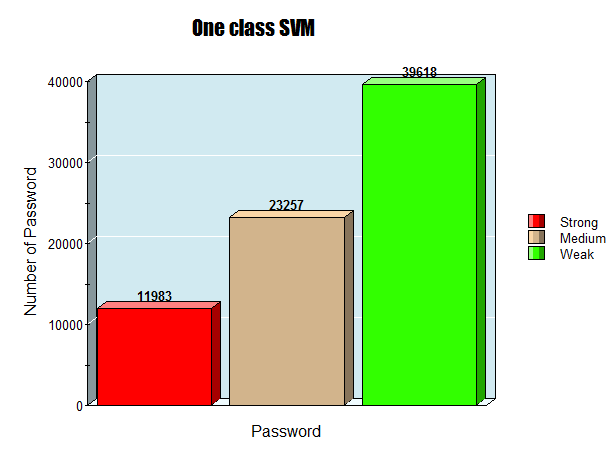
\includegraphics[width=\textwidth]{First.png}
   \end{mdframed}
    \caption{First Experiment.}
  
  \end{minipage}
  
  \hfill
  \centering
  \begin{minipage}[b]{0.4\textwidth}
  \begin{mdframed}
    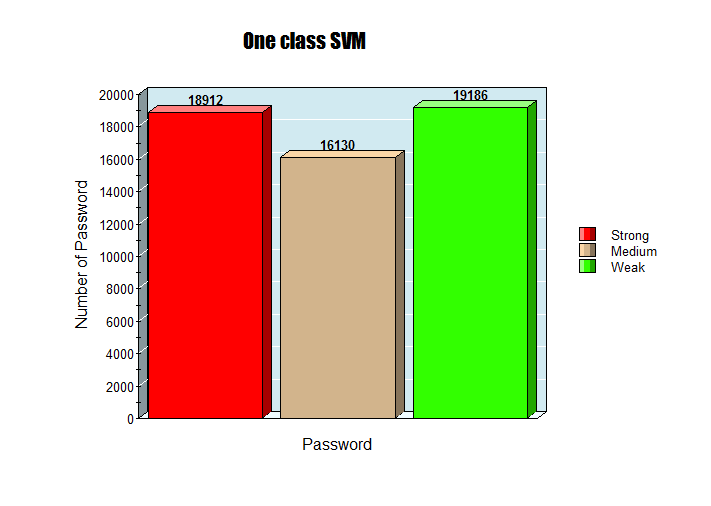
\includegraphics[width=\textwidth]{Secound.png}
\end{mdframed}    
    \caption{Second Experiment.}
  \end{minipage}
  \hfill
  \begin{minipage}[b]{0.4\textwidth}
  \begin{mdframed}
    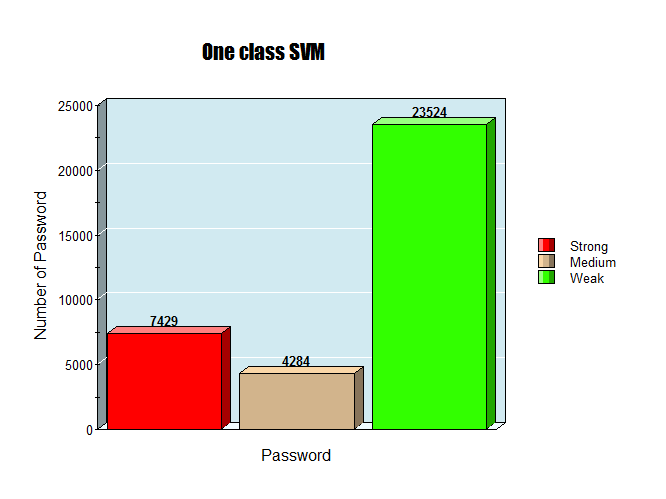
\includegraphics[width=\textwidth]{Third.png}
    \end{mdframed}
    \caption{Third Experiment.}
  \end{minipage}
\end{figure}
\newline
}}
\section{Password Strength Metre:}
{We have created a password strength meter with the help of a one-class support vector machine. With the help of the tool called PARS by Georgia Tech university, we have created a data set of passwords with their strength. We then extracted features from the password. The features are the length of the password, number of vowels, number of special characters, number of the alphabet, number of consonants, and number of numerical. We have done two testings with the data set \par 1. In the first experiment, we have trained the one-class SVM with 70 percent of data set and test with 30 percent of the data set we got an accuracy of 87 percent, but when we added the generated data with data set the accuracy drop to 55 percent it shows that we have successfully created a large subset of a unique password
\par
\begin{figure}
  \centering
\begin{minipage}[b]{0.8\textwidth}
  \begin{mdframed}
    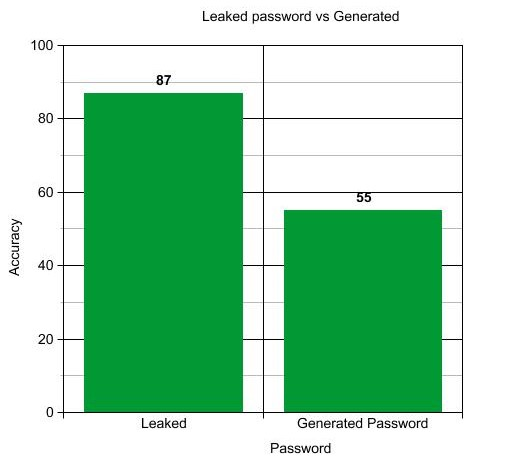
\includegraphics[width=\textwidth]{graph.jpg}
    \end{mdframed}
    \caption{Our Password Strength meter Accuracy}
  \end{minipage}
\end{figure}
\hfill
\par
2. In the second experiment, we give the data set to one class for training. And for testing, we are taking input from the password from the user and provide the strength of the user input password. By comparing it with the available, it is showing the great result.

\begin{table}[htb]
\caption{Few example of One class Support Vector Machine Password Strength Checker}
\begin{tabular}{||c||c||c||c||}
    \hline
    \hline
    \textbf{Password} & \textbf{Existing Meter} & \textbf{Our Model}&\textbf{Remarks} \\
    \hline
    
     \$ANju8820   & Very Strong & Weak & name of user \\
 \hline
 Kundan@#1994  & Very Strong  & Good & name and date of birth \\
 \hline
 JAY!@#882037820  & Very Strong & Good & phone no \\
 \hline
 Bhavendra206 & Strong & Good & simple text\\
 \hline
 8963343643 & Weak & Weak & phone no\\
 \hline
 25081998@devil & Strong & Good & simple\\
 \hline
 lucy@!#9863 & Strong & Weak  & nickname\\
 \hline
 Sirdhar123456!@ & Strong & Good& sequence no\\
 \hline
 lovemysoul & Weak & Weak& simple text\\
 \hline
 liveThelife@1231224 & Strong& Strong& random no\\
 \hline
 netdome8752dxja &Strong &Good& simple text\\
 \hline
 amazon2345da & Good & Good& company\\ 
 \hline
 SANjgaydyatig & Good & Strong& random character\\
 \hline
 Riya@199578fdjy & Strong & Good& name\\
 \hline
 juhiGyani@kichkich & Strong& Strong& name\\
 \hline
 Shikhatek+457674 &Strong & Good& name\\
 \hline
 JyotiKhateN1235 & Strong & Good& name\\
 \hline
 PiyaDon45678 & Strong & Medium& name and dictionary word\\
 \hline
 RiyaJay14758788534 & Strong & Strong& random no\\
\hline
Abcjgdjkash & Weak & Good& random character\\
\hline
123456789 & Weak & Weak& sequence of no\\
\hline
987654321 & Weak & Weak&reverse sequence of number\\
\hline
am1AStrongPassword# & Very Strong & strong& dictionary character\\ 
\hline
11@Mushtehara &Very Strong&good& dictionary character\\
\hline
@nebullae&Very Strong&weak& simple text\\
\hline
!ThereisnoHope12!&Strong&strong& character number and special character \\
\hline
Creator@92&Strong&weak& dictionary word\\
\hline
ds101@iitpnitrkl&Very Strong&strong& combination of everything\\
\hline
som735@iitp&Strong&weak& name of the institute\\
\hline
Xiaomi Redmi Airdots&Strong&medium& company names\\
\hline
joinstar1Q!&Strong&medium& meaningful word\\
\hline
Indianlovesindia@9371&Very Strong&strong& long simple text\\
\hline
xp07DY@?1302_&Very strong&medium& gan created\\
\hline
@Enjoy321#&Very strong&weak&sequence no\\
    \hline
    \hline
\end{tabular}

\end{table}
}

\section{Password suggestion}

\textbf{Password Suggestion: }We all want our system more secure, but as we choose a common word as our password or some dictionary word with some numerical or special character. These leads to easy cracking of the password. To overcome this, we come up with a model that not only checks the strength of the password but also suggests some strong password if the user has chosen a weak password.
\subsection{Overview: }Our model consists of our password strength checker for measuring the strength of the password and BIPASSGAN for generating a new password. The password strength checker model is an extension of the one-class SVM model, which we have trained with the leaked password as well as the password generated by BIPASSGAN.In this model, we have slightly change the BIPASSGAN in which we have taken the weak password, with the information of the user to train our bigan model. Then it sorts the password with their strength score and gives the user top ten strong passwords.

\begin{figure}
  \centering
\begin{minipage}[b]{0.8\textwidth}
  \begin{mdframed}
    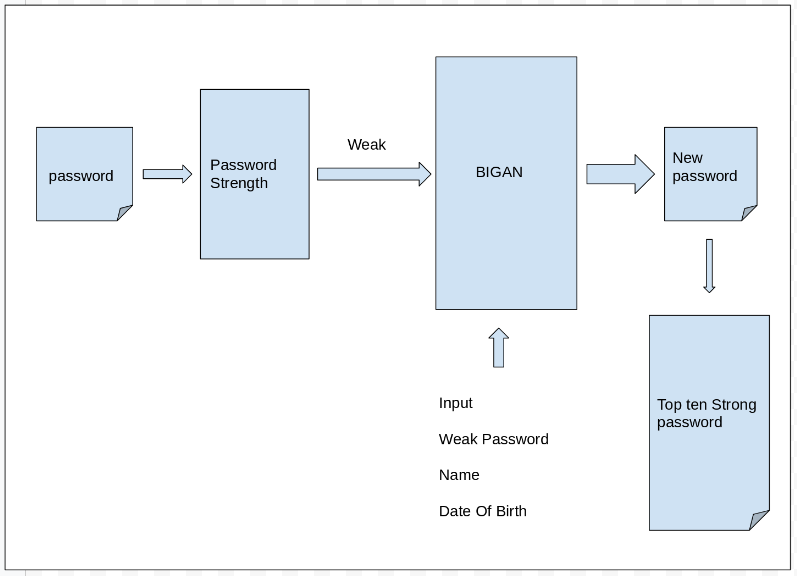
\includegraphics[width=\textwidth]{ab.png}
    \end{mdframed}
    \caption{Our Model}
  \end{minipage}
\end{figure}
\section{Conclusion}

We conclude that though we have pass gan the first deep learning approach for generating a password from the leaked data and we have seen that pass gan has overcome all other generating password technique set but with this new approach \textbf{\quotes{BIPASSGAN}} we have generated a password with less epoch and our generated password is closer to human-created password. So we can conclude that our model is better than pass gan.  We have designed a strength evaluator with the ample amount of passwords generated by bi-pass gan,  that works on the approach of a one-class support vector machine. By comparing it with the available strength meter, we have concluded that our strength evaluator surpasses the available strength meter.

\section{Future Works}
We can use the concept of transfer learning for tuning Bidirectional GAN. As we trained the bi gan model with a large dataset, and it takes a huge amount of time to complete. So we can use the concept of transfer learning to retrain the gan model whenever the new dataset is given. We have used the one-class SVM model for analyzing the strength of the password. Tuning one class SVM can be found as it has only one class, and it hard to optimize the best parameter for the one-class SVM. We can use it for password suggestions. If our one-class SVM predicts that the user password is weak, it will suggest other strong passwords for the user.


% ==================
% # IV. CONCLUSION #
% ==================

%
% ---- Bibliography ----
%
% BibTeX users should specify bibliography style 'splncs04'.
% References will then be sorted and formatted in the correct style.
%
% \bibliographystyle{splncs04}
% \bibliography{mybibliography}
%
%\begin{thebibliography}
%\bibliographystyle{splncs04}
%\bibitem{test}
%fdfd
%\end{thebibliography}

\bibliographystyle{IEEEtran}
\bibliography{bibliography.bib}
\end{document}
